% Replace the contents of this file with your text

\section{Introduction}
\subsection{What is ThermalMonitor?}

ThermalMonitor is an idle task in EFI that allows for temperature tracking and
DUT over-tem\-per\-ature shutdowns. Its goals are to eliminate damage due to
overheating and to allow post-processing of collected temperature data over the
factory lifecycle of a DUT.

\subsection{Motivation}

During the 2014 product cycle it was found that DUTs had been damaged during
the course of production testing due to overheating while in EFI. EFI does not
have CLTM (Closed Loop Thermal Monitor) and did not detect the DUT temperatures
rising beyond their tolerances. The DUTs were heating due to being stacked
inside improperly ventilated trays while in a high power state. Data analysis
concluded that devices from previous years had also seen overheating, but
without the obvious physical manifestations that had occurred during 2014.

\subsection{Document Objective}

This document is generally intended to be an all-around reference for the
consumers and producers of ThermalMonitor and its usage. The goal is to enable
consumers to analyze and diagnose thermal issues in the system using
ThermalMonitor. Although this document will not cover technical details, the
document will explain the design and shed light on the considerations required
to maintain or enhance the software.

\section{Monitoring}
\subsection{Idle Task}

The DUT is considered idle after 500ms of inactivity (no commands running);
otherwise, the DUT is considered busy.

There is no activity in ThermalMonitor while the DUT is busy.  In the idle
state, each available sensor will be polled at a fixed interval.  When
activity occurs on the DUT the ThermalMonitor will stop execution.

It is possible to disable the idle task through DiagsShell. See section
\NumNameRef{sec:UsingThermalMonitor}.

\begin{figure}[!htb]
\begin{center}
	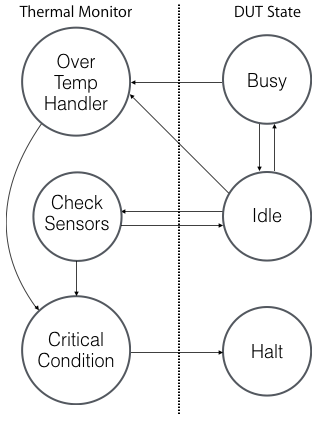
\includegraphics[scale=0.75]{TM_BlockDiagram}

	\caption{ThermalMonitor Block Diagram}
	\label{fig:BlockDiagram}

\end{center}
\end{figure}

\subsection{Sensor Behavior}
\label{sec:SensorBehavior}

Each sensor can have one of three modes:

\begin{Definition}

	\item[Data Collection] There is no temperature limit associated.
	Temperature data will be collected at the preprogrammed interval.
		
	\item[Limit Enabled] Same as Data Collection, but the DUT will shut
	down if the temperature exceeds the configurable limit while the DUT
	is idle.

	\item[Critical Limit] Same as Limit Enabled, but the DUT will shut
	down if the temperature limit is exceeded at any point.

	\begin{itemize}

		\item This is accomplished using temperature interrupts
		associated with each sensor. The interrupts are configured to
		trigger only when an over-temperature event occurs so as not
		to bother busy, normal temperature, DUT.

		\item The interrupt on over-temperature cannot be disabled, but
        the limit can be modified. See section \NumNameRef{sec:ChangingLimits}.

		\item Some sensors are not capable of this configuration and
		cannot be configured to have Critical Limits.

	\end{itemize}

\end{Definition}

Each sensor's mode is predefined in the EFI binary and cannot be changed during runtime.

\subsection{Shutting Down the DUT}
\label{sec:ShuttingDownTheDut}

When a limit is exceeded for either a Limit Enabled or a Critical Limit sensor
the DUT is shutdown in order to prevent damage due to overheating.

Before the DUT can be shutdown, information about the exceeded limit is
recorded.  Due to software limitations, EFI is incapable of saving this
information to a file during the shutdown process. Instead, the information is
stored in the PMU scratch space, which persists across reboot cycles.

Once the event information is stored in the PMU, the DUT is put into its
hibernate state.  Hibernate (S2R) was chosen over Standby (OFF) to allow DUTs
to remain in a low power state while they are attached to the dock connector.

The information stored about the limit failure can be obtained at a later
time.  See section \NumNameRef{sec:ThermalMonitorShutdown}.

\section{Using ThermalMonitor}
\label{sec:UsingThermalMonitor}

\subsection{Data Storage}

Data collected in ThermalMonitor is stored in RAM until it receives
notification to flush to file via internal EFI events. This will occur by
default during shutdown or reset. The data can also be flushed manually by
using the \cmdline{event} command. See section \NumNameRef{sec:SavingData}. If
the internal buffer is full the data will also be flushed. The data will be
appended to the end of the log file and the RAM buffer is reset and emptied.

The contents of the file are in the same CSV format mentioned in section
\NumNameRef{sec:DisplayCollectedTemperatures}.

The file is located on the Log partition. If the Log partition does not exist no
data will persist though reboot. The path to the data file is:

\begin{Setting}
Logs:\MobileMediaFactoryLogs\LogCollector\FactoryDebug\temperature_runtime.csv 
\end{Setting}

\subsection{Commands}

ThermalMonitor also exposes a subset of its functionality through DiagsShell.

\subsubsection{Print Command Line Help}

\begin{CommandLine}
help thermalmonitor
\end{CommandLine}

Print a list of all supported command line options. Not all option combinations are valid.

\subsubsection{Disable ThermalMonitor}

\begin{CommandLine}
thermalmonitor --off
\end{CommandLine}

Disable the ThermalMonitor idle task. No temperature data will be collected unless manually
requested (see section \NumNameRef{sec:ManualTempCheck}). While off the DUT can only will
only be shutdown if a Critical Limit sensor detects an over-temperature event.
See section \NumNameRef{sec:SensorBehavior}.

\subsubsection{Enable ThermalMonitor}

\begin{CommandLine}
thermalmonitor --on
\end{CommandLine}

Enable the ThermalMonitor idle task.  This is the default state of
ThermalMonitor when EFI is started.

\subsubsection{Display Collected Temperatures}
\label{sec:DisplayCollectedTemperatures}

\begin{CommandLine}
thermalmonitor --dump
\end{CommandLine}

Print all temperatures collected since the last time data was flushed to a
file.  The contents of the data buffer will not be changed and data will not be
stored to a file. The output will be in CSV format: 

\begin{Setting}
~\param{<unix\_time>}~, ~\param{<id>}~, ~\param{<dev\_name>}~, ~\param{<temperature>}~
\end{Setting}

Data previously written to the log file will not be show. However, the data
can be displayed using the cat command.

\begin{LogExcerpt}
:-) cat Logs:\MobileMediaFactoryLogs\LogCollector\FactoryDebug\temperature_runtime.csv
1420831170.793s, 0x00, soc, THERMAL0, 27.60
1420831170.793s, 0x01, soc, THERMAL1, 29.00
1420831170.793s, 0x02, soc, CCC_THERMAL0, 27.60
1420831170.793s, 0x03, soc, CCC_THERMAL1, 27.39
1420831170.794s, 0x04, soc, CCC_THERMAL2, 27.39
1420831170.796s, 0x28, pmu, TJINT, 32.63
1420831170.827s, 0x29, pmu, TDEV1, 24.70
1420831170.831s, 0x2A, pmu, TDEV2, 25.46
1420831170.835s, 0x2B, pmu, TDEV3, 25.21
1420831170.839s, 0x2C, pmu, TDEV4, 30.60
1420831194.312s, wrote at: 2015.1.9.19.19.54
\end{LogExcerpt}

\subsubsection{Saving Data to a File}
\label{sec:SavingData}

\begin{CommandLine}
event -s media-sync
\end{CommandLine}

The data that was previously in RAM (displayed via the \cmdline{--dump} option)
will now be store to a file. This is done automatically during shutdown or
reboot.

\subsubsection{Check Temperatures Immediately}
\label{sec:ManualTempCheck}

\begin{CommandLine}
thermalmonitor --check
\end{CommandLine}

Check every available sensor's temperature. If an enabled limit is exceeded,
the DUT will shutdown. Otherwise the command will output all of the newly
collected temperatures in the same format as the \cmdline{--dump} option.

\subsubsection{Change a Sensor Limit}
\label{sec:ChangingLimits}

\begin{CommandLine}
thermalmonitor --dev ~\param{<dev\_name>}~ --name ~\param{<sensor\_name>}~ --setlimit
\end{CommandLine}

Must be used in conjunction with \cmdline{--dev} and \cmdline{--name} in order to select the limit
to update. The below command will set the limit for pmu.TDEV3 to 50. This will only affect Critical
Limit and Limit Enabled sensors.

\begin{LogExcerpt}
:-) thermalmonitor --dev pmu --name TDEV3 --setlimit 50
\end{LogExcerpt}

\subsubsection{Display a Sensor Limit}

\begin{CommandLine}
thermalmonitor --dev ~\param{<dev\_name>}~ --name ~\param{<sensor\_name>}~ --getlimit
\end{CommandLine}

Must be used in conjunction with \cmdline{--dev} and \cmdline{--name} in order to select the limit
to update. The below command will get the limit for pmu.TDEV3.

\begin{LogExcerpt}
:-) thermalmonitor --dev pmu --name TDEV3 --getlimit
Limit TDEV3: 50.000000
\end{LogExcerpt}

\newpage
\subsubsection{List Settings}

\begin{CommandLine}
thermalmonitor --list
\end{CommandLine}

Display a list of available sensors and their settings. The following data will be displayed for each sensor:

\begin{LogExcerpt}
:-) thermalmonitor --list
~\param{<dev\_name>}~.~\param{<sensor\_name>}~:
	SensorId: (~\param{<id>}~)
	Limit: ~\param{<temperature>}~
	Period(ms): ~\param{<period>}~
	Critical: ~\param{<Yes|No>}~
	LimitEnabled: ~\param{<Yes|No>}~
\end{LogExcerpt}

\begin{table}[!htbp]

	\begin{KeywordTable}

		\param{<dev\_name>} & The name of the device the sensor is
		connect to. E.g. "pmu" or "soc". \\

		\param{<sensor\_name>} & The name of the sensor. E.g. "TDEV3"
		or "CCC\_THERMAL1". \\
		
		\param{<id>} & A unique identifier for the sensor. It is generated
        while booting into EFI. The identifier will stay constant across 
        the reboots of the same version of EFI. It can be changed if a new
        sensor gets built into the EFI binary. See section
		\NumNameRef{sec:PostProcessing} for more information on its use. \\

		\param{<temperature>} & User modifiable upper limit of normal
        operating temperature.\\
		
		\param{<period>} & The minimum time between readings
		when the DUT is idle. \\
		
		Critical \param{<Yes|No>} & "Yes" indicates that the sensor has the
		ability to shutdown the DUT on over-temperature events at any
		point.  "No" indicates the DUT must be at idle in order to
		handle over-temperature events. \\

		LimitEnabled \param{<Yes/No>} & "Yes" indicates that an
		over-temperature event will shutdown the DUT. "No" indicates
		that ThermalMonitor will only collect temperature data from
		the sensor. \\

	\end{KeywordTable}

	\caption{Sensor Settings}
	\label{tab:SensorSettings}

\end{table}

\subsection{Updating Default Limits}

The default limits are compiled into the EFI binary and only modifiable by EFI
engineers. The limits should be disabled at the beginning of a product cycle.
Once enough data has been collected the limits should be given to EFI engineers
by the System EE team.

\section{Post-Processing}
\label{sec:PostProcessing}

\subsection{Temperature Data}

Min and max temperature data along with the raw data is uploaded to PDCA at each
restore and log collection station. The raw data can be futher analyzed by a tool
called \cmdline{AnalyzeTemps.py}. If the DUT isn't going through normal factory
process the raw temperature data can be transfered to the host via rsync,
dfufile, usbfs, etc.

\subsection{Using AnalyzeTemps}

The AnalyzeTemps script can be found as an attachment in the following radar:
\newline\href{rdar://problem/19294938}{<rdar://problem/19294938> ThermalMonitor - Scripts and Tools}

\subsubsection{Command Line Summary}

Below is a list of available options when using the tool.

\begin{LogExcerpt}
$ python AnalyzeTemps.py --help
Usage: AnalyzeTemps.py [options]

Options:
  -h, --help            show this help message and exit
  -f FILE, --file=FILE  File containing the temperature data
  -o, --output          print the temperature data
  -p, --plot            plot the temperature data
  -i, --info            Output info about the data
  -d DEV, --device_id=DEV
                        Only use data from this device id
  -t TYPE1,TYPE2,..., --device_type=TYPE1,TYPE2,...
                        Only use data from these device types. pmu, soc, etc
  -n NAME1,NAME2,..., --sensor_name=NAME1,NAME2,...
                        Only use data from these sensor names
  -s START_TIME, --start_time=START_TIME
                        Only use data from this start time
  -e END_TIME, --end_time=END_TIME
                        Only use data up to this end time
\end{LogExcerpt}

\newpage
\subsubsection{Data Summary}

\begin{CommandLine}
python AnalyzeTemps.py -f ~\param{temperature\_runtime\_example.csv}~ -i
\end{CommandLine}

This will print a summary of each sensor recorded in the file.  Below is a
snippet from the output of the command. 

\begin{LogExcerpt}
$ python AnalyzeTemps.py -f temperature_runtime_example.csv -i
~\elide~
pmu.TDEV3:
	Num samples: 141
	First sample time: 1418399046.660 (2014-12-12 10:44:06)
	Last sample time: 1418760241.201 (2014-12-16 15:04:01)
	Min temperature: 23.94
	Min temperature time: 1418753746.572 (2014-12-16 13:15:46)
	Max temperature: 46.64
	Max temperature time: 1418760241.201 (2014-12-16 15:04:01)
~\elide~
\end{LogExcerpt}

The temperatures will be displayed in the units they were collected in. Units
are not stored in the file, so they are not displayed. The timestamps are
dependant on the programmed value in the RTC. Usually this is programmed to GMT.
 
\subsubsection{Limiting the Results}

The results can be further narrowed down via time, device ID, device name, or sensor name. 

\begin{CommandLine}
python AnalyzeTemps.py -f ~\param{FILE}~ -o -t ~\param{pmu}~ -n ~\param{TDEV4}~ -s ~\param{1418760127}~
\end{CommandLine}
 
This command filters the output to be from sensors attached to the PMU named
TDEV4. The results are further reduced by filtering out all the data points
before the specified start time. The \cmdline{--start-time} option should be
in Unix time and can be translated into human readable format via
an online tool\footnote{\url{http://www.epochconverter.com}}.

\newpage 
\subsubsection{Plotting Data}

The data can also be plotted using the same tool. The plot will display on the
host in a separate window from the terminal. 

\begin{CommandLine}
python AnalyzeTemps.py -f ~\param{temperature\_runtime\_example.csv}~ -p
\end{CommandLine}

\begin{figure}[!htb]
\begin{center}
	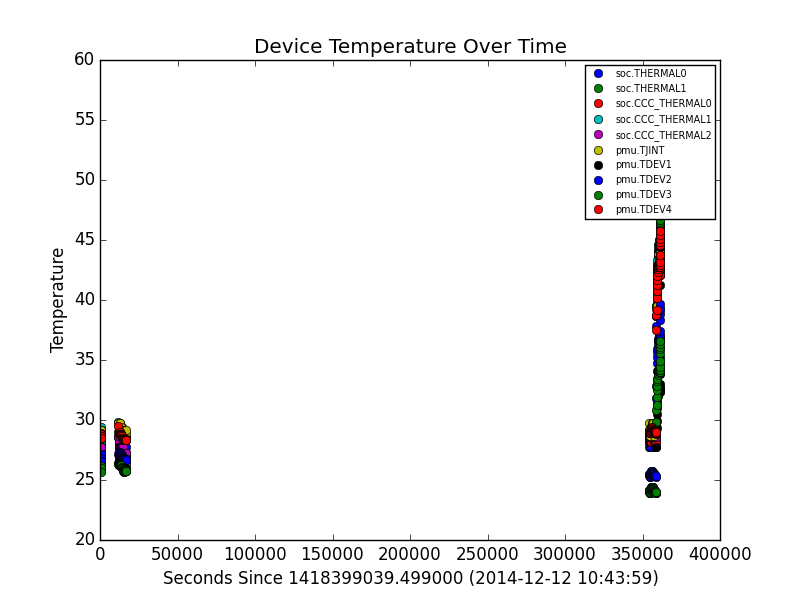
\includegraphics[scale=0.75]{BasicPlot}

	\caption{Basic Temperature Plot}
	\label{fig:BasicTemperaturePlot}

\end{center}
\end{figure}

\newpage 
\subsubsection{Plotting Filtered Results}
The plotting functionality also works with the filtering options.

\begin{CommandLine}
python AnalyzeTemps.py -f ~\param{temperature\_runtime\_example.csv}~ -p -t ~\param{pmu}~ -s ~\param{1418750040}~
\end{CommandLine}

\begin{figure}[!htb]
\begin{center}
	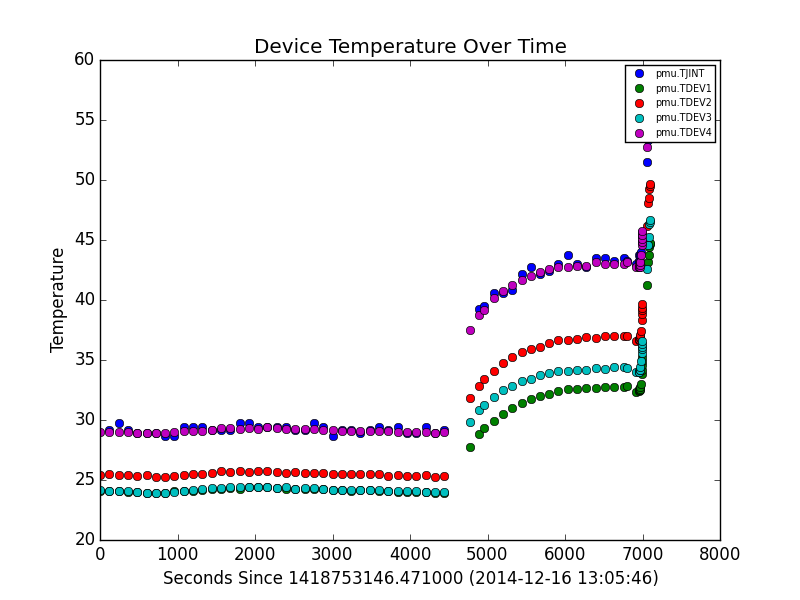
\includegraphics[scale=0.75]{DeviceTypeStarting}

	\caption{Filtered Temperature Plot}
	\label{fig:FilteredTemperaturePlot}

\end{center}
\end{figure}

\newpage 
\subsection{PDCA Parametric Data}

The PDCA keys are in the following format:

\begin{Setting}
~\param{<MAX\_TEMP|MIN\_TEMP>}~.~\param{<dev\_name>}~.~\param{<sensor\_name>}~
\end{Setting}

For example, the maximum GasGauge termperature can be found via key:

\begin{Setting}
~\param{MAX\_TEMP}~.~\param{battery}~.~\param{GasGauge}~
\end{Setting}

Min and max data are reset after each restore. The parametric data is uploaded
at each restore station so no data is lost. The data is uploaded using the
station ID of the corresponding restore or log collection station.

\subsection{ThermalMonitor Shutdown}
\label{sec:ThermalMonitorShutdown}
As mentioned in section \NumNameRef{sec:ShuttingDownTheDut}, the ThermalMonitor task will save
critical data about the sensor that exceeded the temperature threshold before
the DUT is shutdown. During a subsequent entry into EFI, this information
is moved from the PMU to a file. The file is located in the following location:

\begin{Setting}
Logs:\MobileMediaFactoryLogs\LogCollector\FactoryDebug\shutdown.log
\end{Setting}

If an over-temperature shutdown occurs, a BootStageDebugThermal entry will be
appended to the end of the file with the following format: 

\begin{LogExcerpt}
Type: BootStageDebugThermal
	Time: 2014-12-15 19:04:17
	CommitId: CA30
	SensorId: 0x2C
	TempC: 23.25
	LimitC: 20.00
\end{LogExcerpt}

\section{Future Work}

\subsection{Radars}

\href{rdar://problem/19179025}{<rdar://problem/19179025> Convert Sochot to be a
thermal event with ThermalMonitor}\newline
SocHot is a separate mechanism in EFI and should be merged with the
ThermalMonitor

\href{rdar://problem/19432841}{<rdar://problem/19432841> Make ThermalMonitor
post processing scripts available in the non-ui SDK}\newline
Make obtaining the post processing script easier.
